\documentclass{article}

\usepackage[margin=1in]{geometry}
\usepackage{graphicx}
\usepackage{amsmath,amssymb}
\usepackage{url}
\usepackage{hyperref}
\usepackage{caption}
\usepackage{subcaption}

\graphicspath{{figures/}}

\title{Pitfalls and Lessons: Zero-Shot Failures in Symbolic Generalization}
\author{
  Ambitious AI Researcher \\
  \texttt{air@researchlab.ai}
}
\date{}

\begin{document}

\maketitle

\begin{abstract}
Zero-shot generalization often fails when models face symbolic or systematic configuration changes, leaving real-world deployments at risk. We investigate these pitfalls by analyzing how certain representational and preprocessing choices exacerbate or mitigate our models' inability to extrapolate. We highlight negative or inconclusive findings that warn practitioners about hidden assumption mismatches.
\end{abstract}

\section{Introduction}
Large-scale neural models sometimes appear to master tasks yet break down on slightly altered inputs that require symbolic inference. Even as models improve on standard benchmarks, real-world use cases demand robust extrapolation. Our study reveals deep pitfalls in zero-shot performance and partial successes in certain ablations. By focusing on negative results, we aim to steer future work toward safer and more reliable architectures.

We first discuss how prior work addresses symbolic tasks yet fails to fully capture subtle context shifts. We then detail our setup, baselines, and targeted ablations. Our experiments show consistent underperformance when token-level structure changes, even while in-domain metrics remain high. We conclude with insights that can guide researchers away from brittle generalizations.

\section{Related Work}
Prior studies on systematic generalization often point to the inability of deep networks to capture compositional structure \cite{lake2018generalization, loula2018arr, bastings2018jump}. Data augmentation and specialized architectures attempt to alleviate these shortcomings \cite{andreas2019good, keysers2020measuring}, but strong improvement remains elusive \cite{ontanon2022making}. Recently, attempts to mix rule-based systems with neural networks have shown partial promise \cite{liu2020compositional}, though brittle edge cases remain frequent \cite{gulordava2018colorless}.

\section{Method / Problem Discussion}
We explore sequence-to-sequence tasks designed to evaluate symbolic manipulation. Our baseline uses an encoder-decoder Transformer with standard embeddings. We focus on zero-shot performance under token substitutions or partial reorderings. We introduce random token masking, freezing embeddings, and one-hot representations as ablations to test the trade-off between lexical-level memorization and generalization.

\section{Experiments}
We train on synthetic data with consistent symbol rules and test on held-out symbol configurations. We find standard models yield high in-domain accuracy but fail to extrapolate. Figure~\ref{fig:main_figure} provides training and validation curves alongside zero-shot results for baselines and ablations. The gap highlights models' lack of symbolic compositionality.

\begin{figure}[t]
  \centering
  \includegraphics[width=0.7\linewidth]{main_multisub.png}
  \caption{Training and validation performance vs.\ zero-shot results across multiple ablations. Despite similar training accuracy, zero-shot performance is considerably worse.}
  \label{fig:main_figure}
\end{figure}

When random token masking is introduced, zero-shot performance deteriorates further, suggesting that lexical memorization alone drives model success. See Appendix for additional figures illustrating the impact of these ablations.

\section{Conclusion}
We investigated why zero-shot generalization remains fragile in symbolic tasks. Our negative results highlight the perils of relying on superficial patterns. Future work should address structural biases and test robustly for out-of-distribution symbolic shifts. Our findings may guide both dataset creation and architecture design to reduce brittleness.

\clearpage
\appendix

\section{Appendix: Extended Results}
Figure~\ref{fig:random_token_mask15} shows how random token masking severely degrades performance. Figure~\ref{fig:embedding_comparison} contrasts frozen embeddings and one-hot representations, neither of which resolves the zero-shot gap.

\begin{figure}[h]
  \centering
  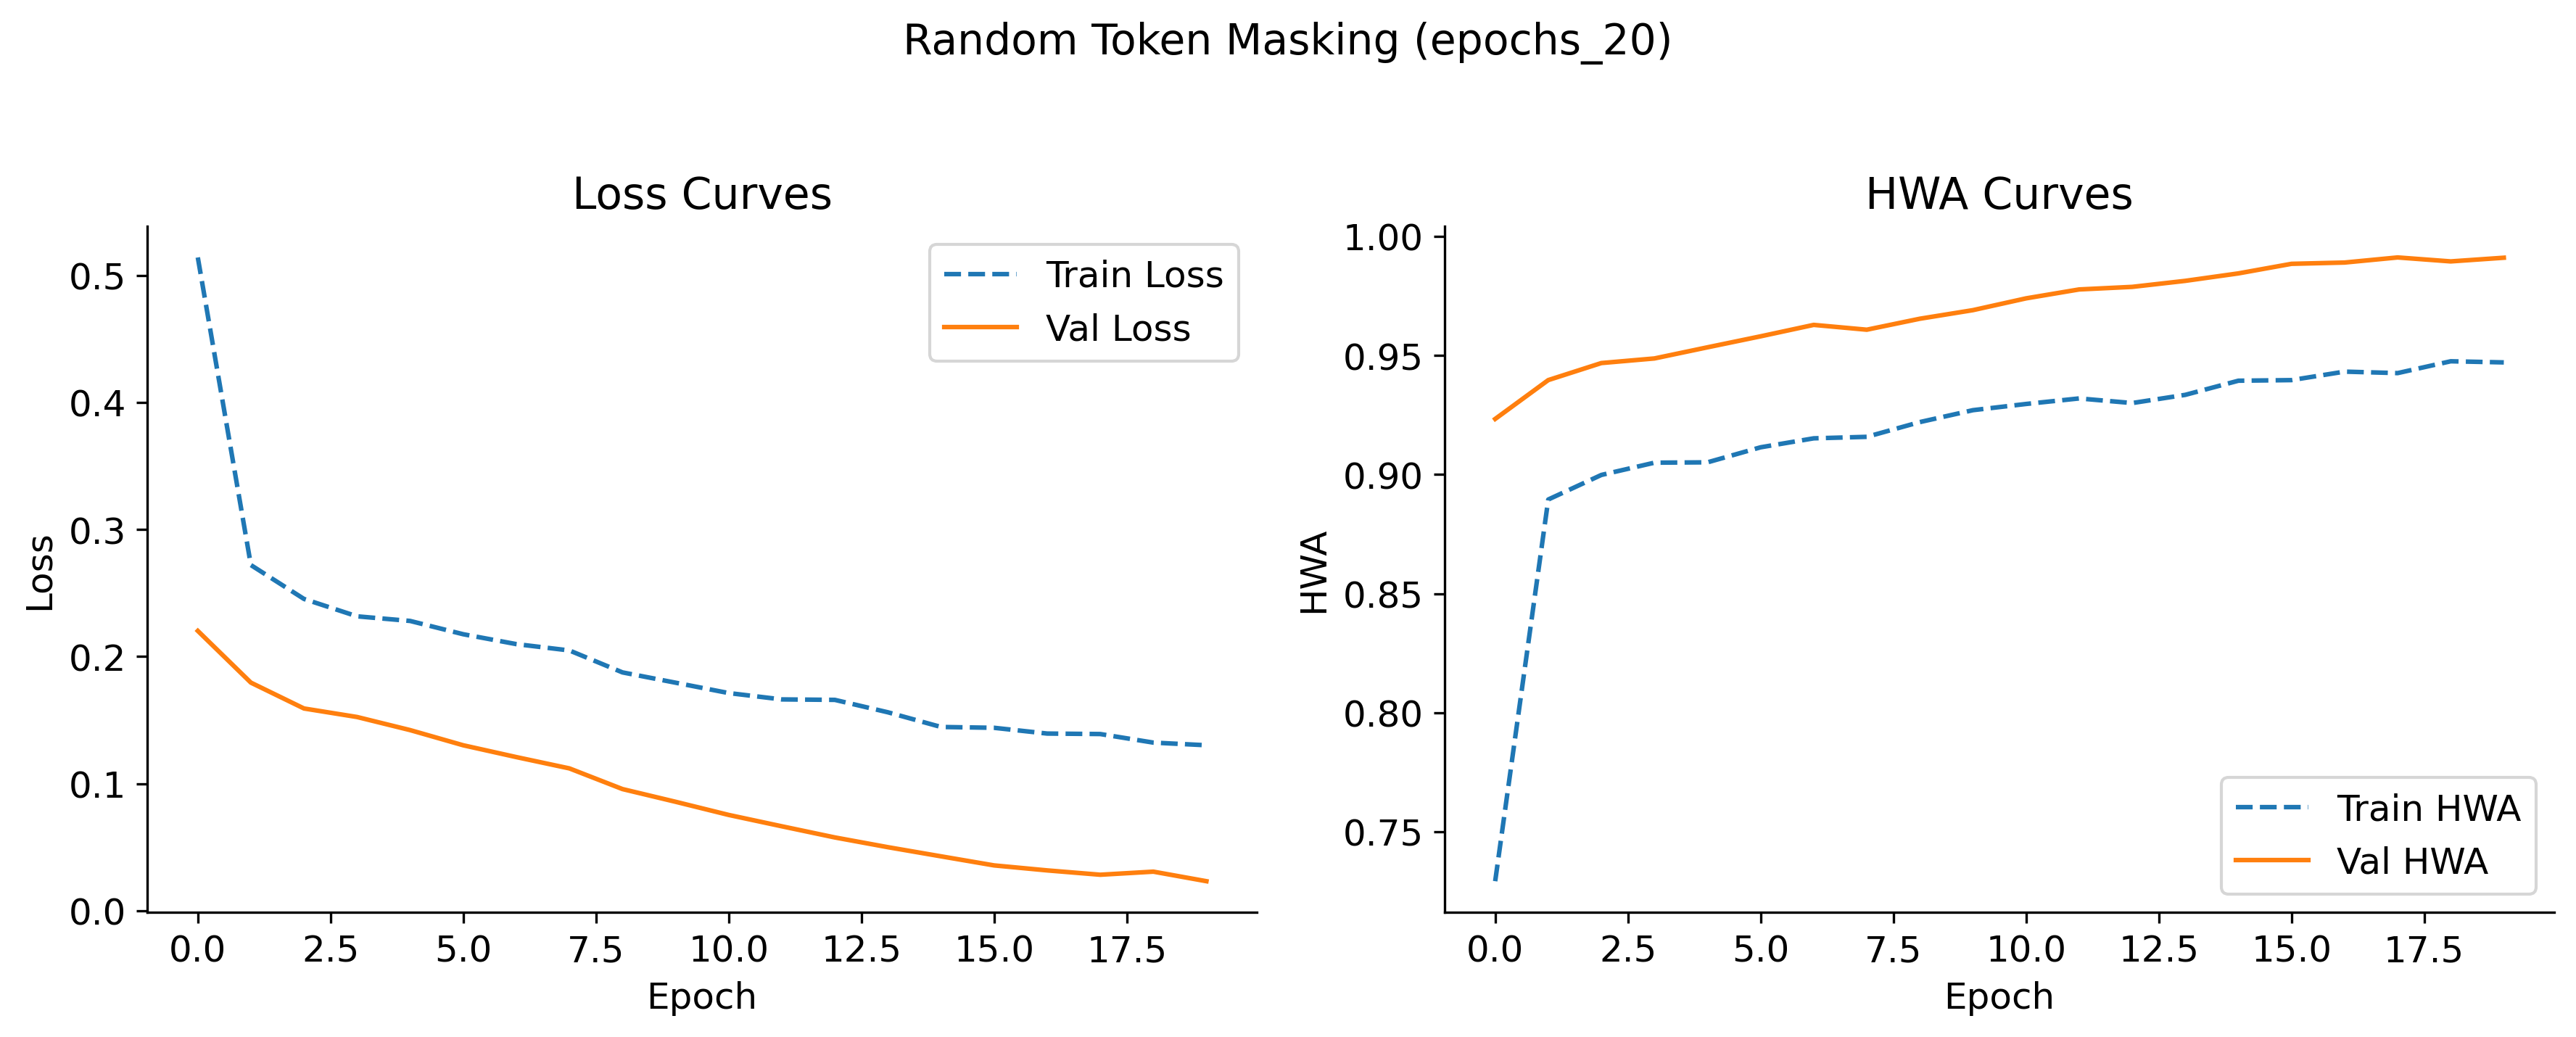
\includegraphics[width=0.45\linewidth]{random_token_mask_15.png}
  \caption{Exacerbated performance drop under random masking.}
  \label{fig:random_token_mask15}
\end{figure}

\begin{figure}[h]
  \centering
  \begin{subfigure}{0.45\linewidth}
    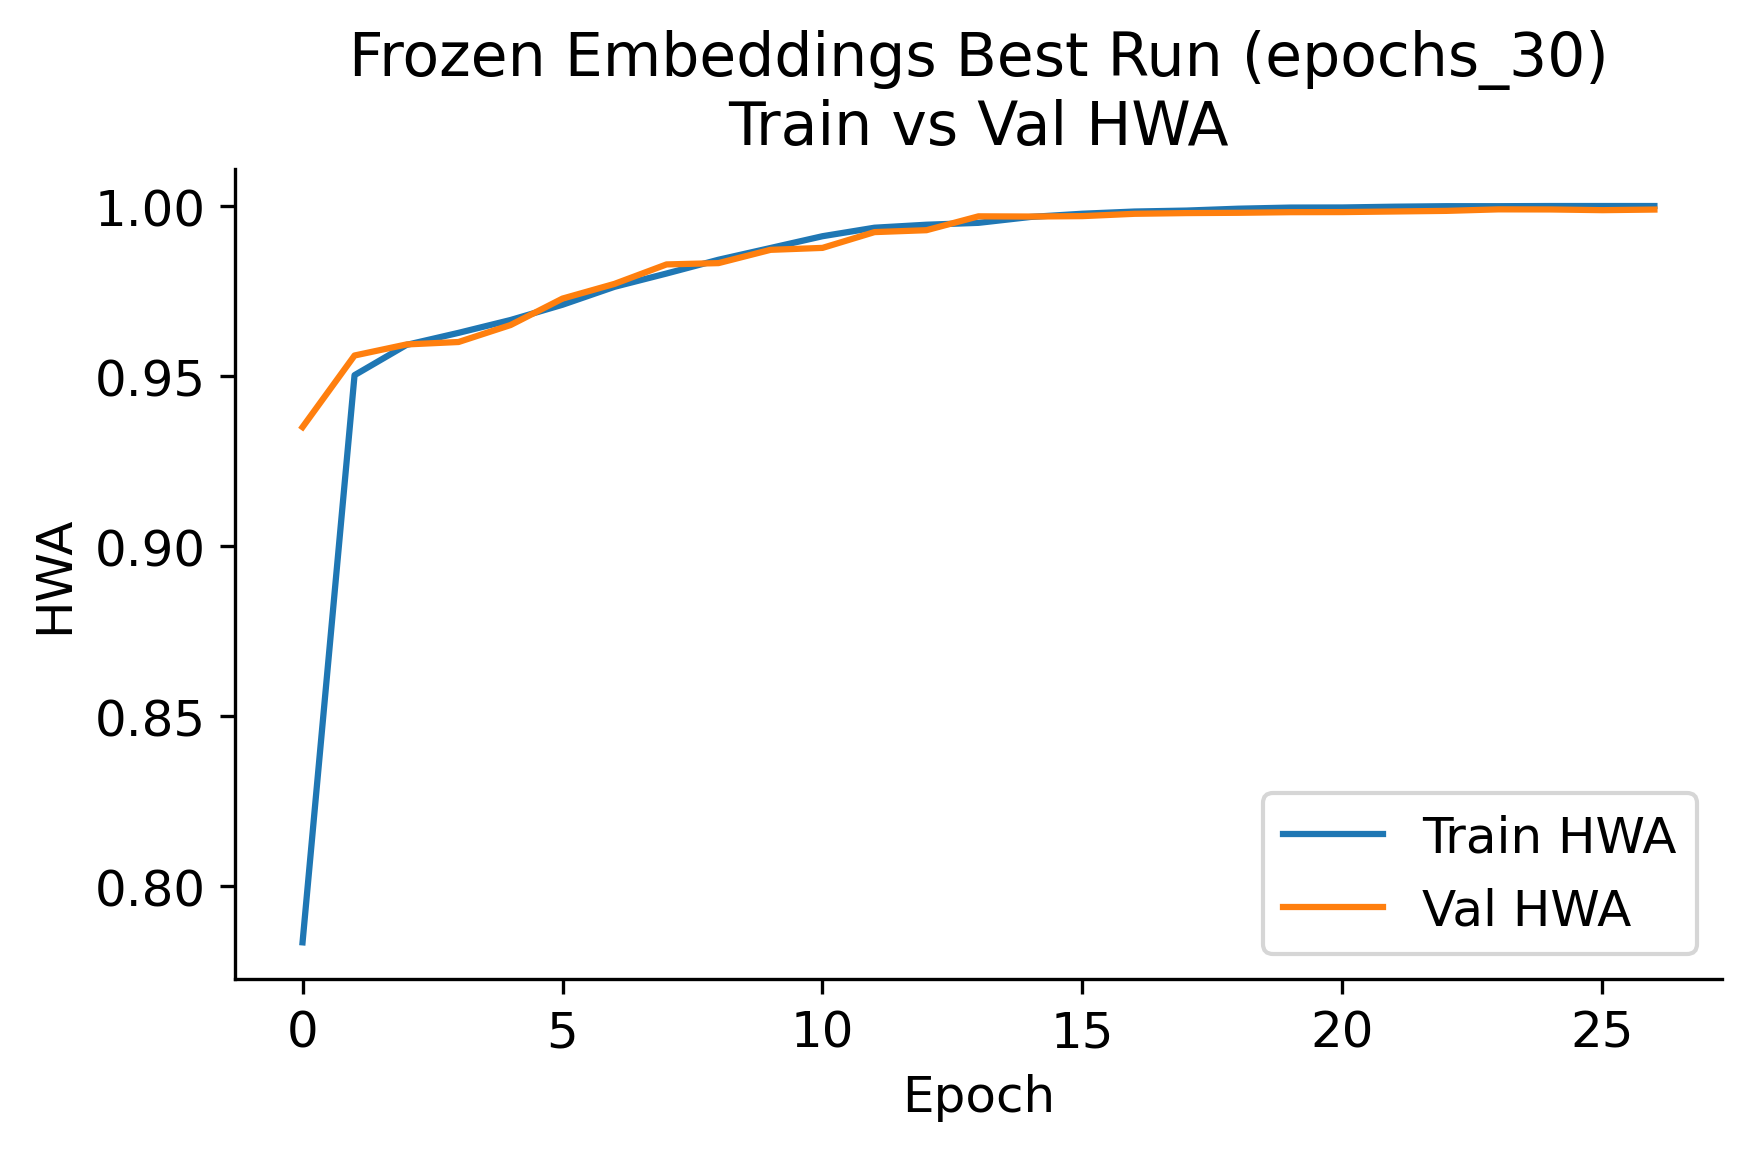
\includegraphics[width=\linewidth]{frozen_embeddings_best_hwa.png}
  \end{subfigure}
  \quad
  \begin{subfigure}{0.45\linewidth}
    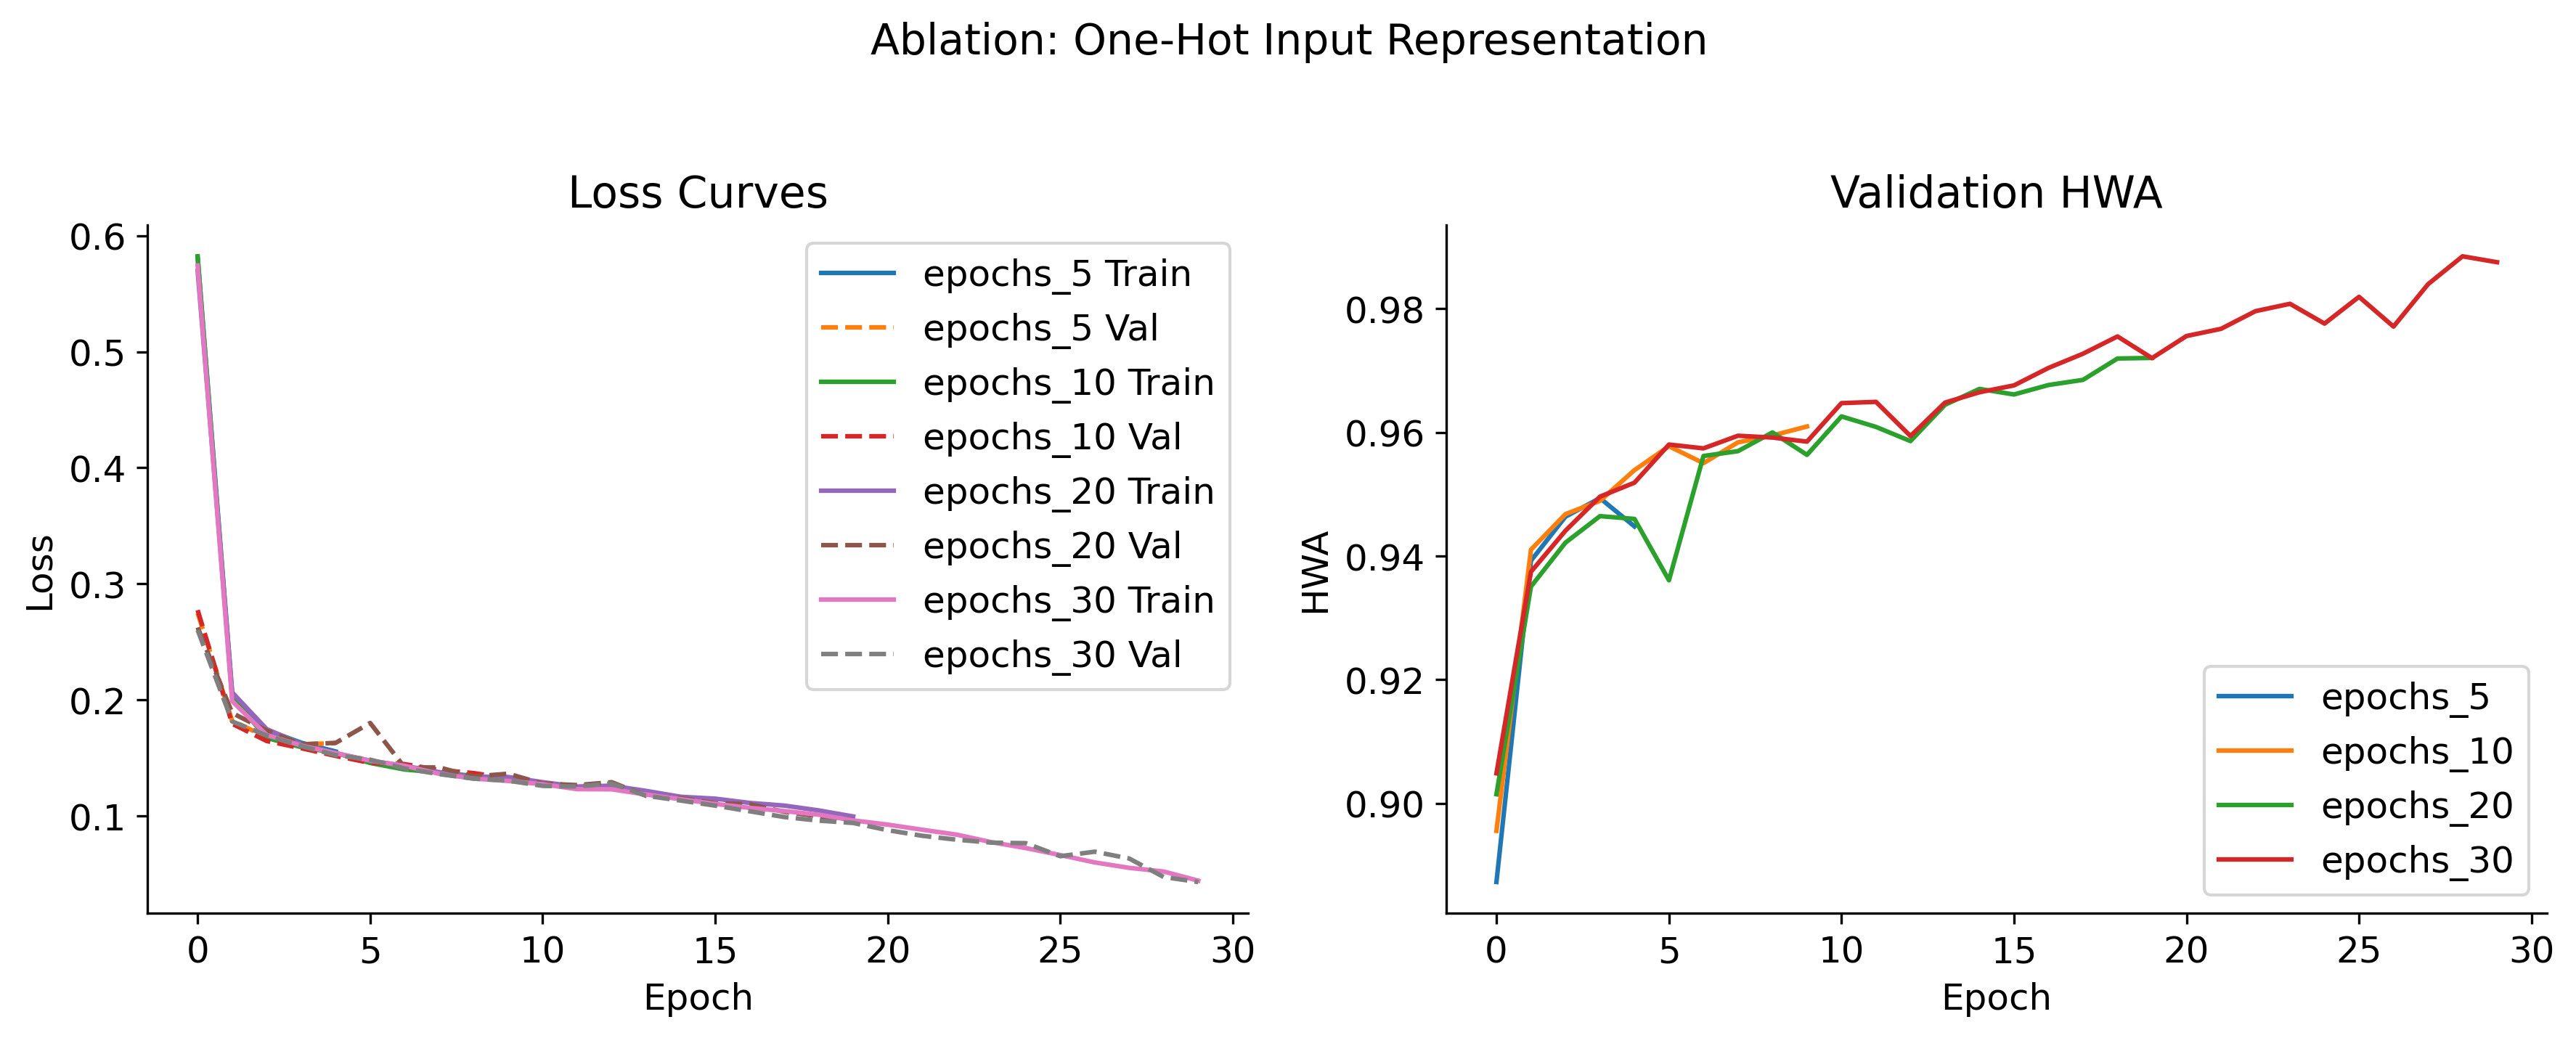
\includegraphics[width=\linewidth]{onehot_no_embedding.png}
  \end{subfigure}
  \caption{Frozen embeddings and one-hot representations did not significantly lessen zero-shot failures.}
  \label{fig:embedding_comparison}
\end{figure}

\clearpage

\begin{filecontents}{references.bib}
@inproceedings{lake2018generalization,
  title={Generalization without Systematicity: On the Compositional Skills of Sequence-to-Sequence Recurrent Networks},
  author={Lake, Brenden M and Baroni, Marco},
  booktitle={ICML},
  year={2018}
}

@inproceedings{loula2018arr,
  title={Rearranging the Familiar: Testing Compositional Generalization in Recurrent Networks},
  author={Loula, Jo\~ao and Baroni, Marco and Lake, Brenden M},
  booktitle={BlackboxNLP Workshop at EMNLP},
  year={2018}
}

@inproceedings{bastings2018jump,
  title={Jump to Better Conclusions: SCAN Both Left and Right},
  author={Bastings, S. and Lake, B. and Baroni, M.},
  booktitle={Workshop on Analyzing and Interpreting Neural Networks for NLP},
  year={2018}
}

@inproceedings{andreas2019good,
  title={Good-Enough Compositional Data Augmentation},
  author={Andreas, Jacob},
  booktitle={ACL},
  year={2019}
}

@article{keysers2020measuring,
  title={Measuring Compositional Generalization: A Comprehensive Method on Realistic Data},
  author={Keysers, Daniel and et al.},
  journal={Transactions of the ACL},
  year={2020}
}

@inproceedings{ontanon2022making,
  title={Making Systematic Generalization More Systematic in Instruction Following Tasks},
  author={Ontan{\'o}n, Santiago},
  booktitle={NeurIPS},
  year={2022}
}

@inproceedings{liu2020compositional,
  title={Compositional Generalization via Neural-Symbolic Stack Machines},
  author={Liu, Felix and et al.},
  booktitle={ICLR},
  year={2020}
}

@inproceedings{gulordava2018colorless,
  title={Colorless Green Recurrent Networks Dream Hierarchically},
  author={Gulordava, Kristina and et al.},
  booktitle={NAACL-HLT},
  year={2018}
}
\end{filecontents}

\bibliographystyle{abbrv}
\bibliography{references}

\end{document}